\documentclass[11pt,a4paper]{article}
\usepackage[T1]{fontenc}
\usepackage[latin1]{inputenc}
\usepackage{a4wide}
\usepackage{lmodern}
\usepackage{float}
\usepackage[dvips]{graphicx}

\usepackage[
pdfauthor={ACE Project Team},
pdftitle={System Requirements},
pdfcreator={pdftex},
]{hyperref}

\usepackage{sectsty}
\allsectionsfont{\sffamily}

\usepackage{fancyheadings} 
\pagestyle{fancy} 
\lhead{\textsf{\textbf{ACE} \\ \small{a collaborative editor}}}
\chead{}
\rhead{
\parbox[c]{3cm}{
\includegraphics[height=0.875cm,width=3cm]{../../images/logo_BFH.eps}}
\parbox[c]{2.2cm}
{\tiny{\textsf{Berner Fachhochschule \\
Hochschule f�r \\
Technik und Informatik}}}}
\lfoot{}
\cfoot{\textsf{\thepage}}
\rfoot{}
\setlength{\headrulewidth}{0.6pt}
\setlength{\footrulewidth}{0.6pt}
\setlength{\topmargin}{-50pt}
\addtolength{\headheight}{50pt}

\usepackage{colortbl}

\newcommand{\headercol}[2]{\multicolumn{1}{|>{\bfseries\columncolor[gray]{0.82}}p{#1}|}{\textsf{#2}}}
\newcommand{\ace}[0]{\emph{ACE }}



\begin{document}

\setlength{\parindent}{0pt}

\begin{titlepage}
\thispagestyle{empty}
  
\includegraphics[height=1.5in]{../images/pix.eps}

  \begin{center}

    {\fontsize{40}{45} \textbf{\textsf{ACE}}} \\
    \textsf{a collaborative editor} \\
        
    \vspace{36pt}
        
    {\huge{\textbf{\textsf{}}}} \\

    \vspace{36pt}

	\textsf{Berne University of Applied Sciences} \\
    \textsf{School of Engineering and Information Technology} \\
    
  \end{center}

  \vfill
  
  \begin{tabular}{ll}
   \hline

   \\

   \multicolumn{1}{>{\bfseries}p{1.5in}}{\textsf{Date:}} &
   \multicolumn{1}{>{}p{4.3in}}{\textsf{08.11.2005}}          \\
   
   \\
   
   \multicolumn{1}{>{\bfseries}p{1.5in}}{\textsf{Version:}}     &   
   \multicolumn{1}{>{}p{4.3in}}{\textsf{0.1}}                 \\

   \\
   
   \multicolumn{1}{>{\bfseries}p{1.5in}}{\textsf{Projectteam:}}                 &
   \multicolumn{1}{>{}p{4.3in}}{\textsf{Mark Bigler (biglm2@hta-bi.bfh.ch)}}  \\
   \multicolumn{1}{>{\bfseries}p{1.5in}}{}                                      &
   \multicolumn{1}{>{}p{4.3in}}{\textsf{Simon Raess (rasss@hta-bi.bfh.ch)}}    \\
   \multicolumn{1}{>{\bfseries}p{1.5in}}{}                                      &
   \multicolumn{1}{>{}p{4.3in}}{\textsf{Lukas Zbinden (zbinl@hta-bi.bfh.ch)}} \\   
   
   \\
   
   \multicolumn{1}{>{\bfseries}p{1.5in}}{\textsf{Receivers:}}                       &
   \multicolumn{1}{>{}p{4.3in}}{\textsf{Jean-Paul Dubois (doj@hta-bi.bfh.ch)}}       \\
   \multicolumn{1}{>{\bfseries}p{1.5in}}{}                                          &
   \multicolumn{1}{>{}p{4.3in}}{\textsf{Claude Fuhrer (frc@hta-bi.bfh.ch)}}       \\

   \\
   
   \multicolumn{1}{>{\bfseries}p{1.5in}}{\textsf{Location:}}               &   
   \multicolumn{1}{>{}p{4.3in}}{\textsf{Subversion Repository}} \\

   \\  
   
   \hline
  \end{tabular}

\end{titlepage}


\tableofcontents
\newpage


\section{Introduction}

The \emph{System Requirements} document lists the goals and desired 
functionality of ACE.


\section{Project Goals}

The goal of the project ACE is to create a collaborative text editor. In 
the following a more detailed description of the functionality is described.
The project goals are categorized into mandatory, optional, and non-goals.

\subsection{Mandatory Goals}
The following list shows the basic features of the text editor.
\begin{itemize}
 \item create new documents
 \item load and save documents
 \item open multiple documents at the same time
 \item switch between open documents
 \item cut/copy/paste
 \item about information
\end{itemize}

This is the list of collaboration functionality that must be implemented.
\begin{itemize}
 \item publish local documents
 \item automatic discovery of other running instances of ACE on a local area network
 \item automatic discovery of published documents of other running instances of ACE
 \item join published documents
 \item collaborative editing in a shared document
 \item awareness information
 \item leave joined documents
 \item kick users
 \item conceal published documents
\end{itemize}

\subsubsection{Publishing Documents}
Local documents can be published. These published documents are discovered by other
running instances of ACE.

\subsubsection{Discovery}
Running ACE instances as well as published documents have to be discovered on the local
area network automatically.

\subsubsection{Joining Sessions}
Discovered shared documents of other users can be joined. When another document is
joined successfully, the user can edit the joined document in collaboration with the
other users already part of that editing session.

\subsubsection{Collaborative Editing}
When a shared document is joined, it is possible to collaboratively edit the 
same shared document at the same time. 

\subsubsection{Awareness Information}
So-called awareness information provides information about the other users editing location, 
i.e. their current text insert position and selection. This awareness information
helps to avoid that two users are editing the same document location.

\subsubsection{Leaving Sessions}
Already joined document editing sessions can be left voluntarily by the users or they
can be kicked from the session by the publisher (e.g. if the user is not behaving well).

\subsubsection{Conceal Document}
A publisher of a document can conceal a document, which effectively ends the collaborative 
editing session. 


\subsection{Optional Goals}

We might implement optional goals if we have additional time.

\begin{itemize}
 \item access right mechanism
 \item manual discovery of running instances outside of the local area network
 \item invite other users to a session 
\end{itemize}

\subsubsection{Access Right Mechanism}

There is no mandatory goal that requires any kind of access right mechanism 
meaning that any user can join a published document and gain read/write 
access. Of course, this can be an undesirable situation, especially in an 
environement where you do not trust all the other users on the local 
area network.

An access right mechanism should allow the publisher to choose default access 
rights for each of his published documents. These default access rights 
specify which access rights a freshly joined user gets. Reasonable access 
modes would be:

\begin{itemize}
 \item ask for join permission
 \item read-only access
 \item read-write access
\end{itemize}

The first access mode ensures that nobody can access or even view a shared 
document before the publisher explicitely grants that user more the permission
(i.e. read-only or read-write). The access rights can be changed for each 
user independently or globally for all participants in a shared document.

\subsubsection{Manual Discovery}

Beside the automatic discovery, a mechanism to explicitely discover other users
might be implemented. This mechanism allows to enter IP/port information to
connect to another ACE instance running on another network.

\subsubsection{Invitations}
The publisher of a shared document should be able to invite other users to an 
editing session of a particular shared document.

\subsection{Non-Goals}

Due to the limited available time, certain (useful) functionality cannot be 
implemented in the diploma project. The principle is that if something is not
explicitely listed in the project goals, it is not a goal of the project. 
However, we want to explicitely highlight in this section some points that are 
not goals.

\begin{itemize}
 \item security aspects: authentication, confidentiality
 \item undo/redo
\end{itemize}

\subsubsection{Security Aspects}
Collaborative editing requires that changes to the local replica of the shared 
document must be sent to the other participants. These changes pass through
the network and thus can be viewed by eavesdroppers. As the document might 
contain potentially confidential information, ideally all transformation 
should be encrypted.

Further, if a user tries to join a document, the publisher should be certain 
who the joining user is. The use of digital signatures would help to 
ascertain the identity of the joining user.

Although both authentication and confidentiality would be very useful additions
to a collaborative editor, they will not be implemented in ACE for time 
reasons.

\subsubsection{Undo/Redo}
In the semester project we envisioned ACE to have a fully functioning 
undo/redo, even in a collaborative editing session. Unfortunately we have 
stumbled across a bug, which we could not resolve in reasonable time. That is 
the reason why ACE will not have any undo/redo actions. We will explain the 
source of the problem in detail in the final report. 


\newpage
\section{Requirements}

In this section, the basic requirements for ACE are described.

\subsection{Platform Independence}
The currently only working collaborative text editor is limited to the Mac
platform. ACE must run on at least Windows, Linux, and Mac platform.

\subsection{Programming Language}
ACE has to be implemented with Java SE 1.4.2. This requirement comes directly
from the platform independece requirement.

\subsection{Interoperability}
The protocol employed by ACE should be open and platform independent. 
For that reason, we won't use Java serialization in the network layer.

\subsection{Configuration}
As ACE is an end-user application, the required configuration for the application should be 
minimal, ideally zero. Most users will feel lost if they have to enter IP addresses 
and ports. So ACE has to support automatic discovery of other users (other running instances 
of ACE) and their shared documents.

\subsection{No Server Application}
ACE is an end-user application. We do not want that it is necessary to setup
an additional server application in order to use ACE. All that should be
necessary to start using ACE is to download the application and start it.


\newpage
\section{Functionality}

In this section some functionality not obviously described in the goals section
is presented.

\subsection{Documents View}
It must be possible to switch between open documents. The document switcher must
convey the kind of document: local, published, remote. A
\emph{local} document is only visible and editable by the local user. A
\emph{published} document is published by the local user and can be joined by
other users. A \emph{remote} document is a published document from another
user joined by the local user.

\subsection{Browse View}
In the GUI, all published documents of other users whose instance of ACE
is running on the local area network must be visible in a discovery browser
view. From this discovery browser it must be possible to join shared documents.
The publisher of the document is also displayed alongside the document name.

\subsection{Participant View}
For a published or a remote document, a list of all the participants in the
collaborative editing session must be displayed in the GUI. This view is
automatically updated whenever a user joins or leaves the editing session.


\newpage
\section{Architecture}

ACE uses a concurrency control algorithm that is based on a client-server 
architecture. The document content is replicated at each participant's
site. In order to maintain the consistency of the replicas, each locally
generated operation (e.g. insert/delete) has to be sent to the server. The
server transforms the incoming operation and forwards it to all the other
pariticipants in the editing session. This architecture has some significant
advantages. First, it is a natural fit for collaborative editing. A user shares 
a local document and other users can join the editing session. Naturally, the
publisher plays the role of the server in the editing session. Second, it
simplifies the implementation and complexity of the network layer. Clients
have to open a connection to the server only and all operations are sent only
directly to server (instead of sending it to all other participants directly).

In ACE, each running instance of the application will start one network level
server. This server publishes the presence of the application on the local
area network. It runs inside the client application. There is no specialized 
server application running on another host.

For each published document an additional logical server exists for the 
transformation and forwarding of messages. This logical server is not an 
additional network server. There will be only one well-known server
socket running per application.

In figure \ref{fig:session} you see an editing session with one publisher 
and three participants ($C_{1}$, $C_{2}$, and $C_{3}$). In the picture on
the left you see that participant $C_{1}$ sends an operation to the
session's logical server component running inside the publisher's application.
The logical server transforms the incoming operation against other concurrent
operations (there are none in this figure) and forwards it to all other
participants, including to the publisher that is running inside the same
application.

\begin{figure}[H]
 \centering
 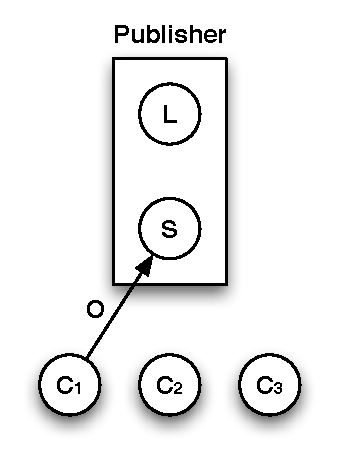
\includegraphics[width=5.18cm,height=7.26cm]{../images/session-1.eps}
 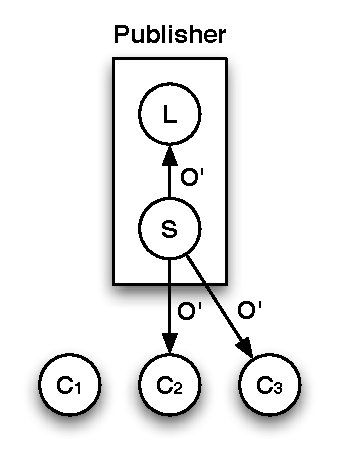
\includegraphics[width=5.18cm,height=7.26cm]{../images/session-2.eps}
 \caption{Logical View of an Editing Session}
 \label{fig:session}
\end{figure}

The situation above consisted of the situation with one session. Of course, 
one application can play the role of the publisher and of participant 
multiple times. The figure \ref{fig:collaboration} shows a network with three 
applications. User C shares document 1 and user A shares documents 2 and 3. 
Each user in this situation is part of the documents 1, 2, and 3, either as 
publisher or as participant.

\begin{figure}[H]
 \centering
 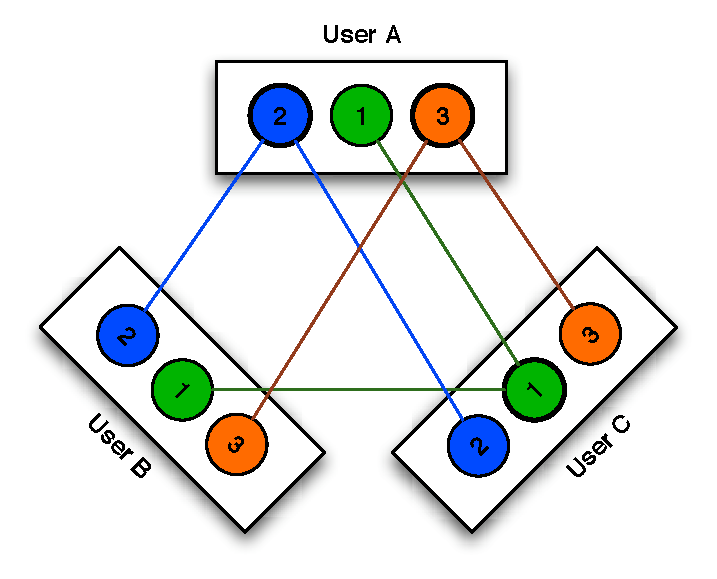
\includegraphics[width=11.57cm,height=9.24cm]{../images/collaboration.eps}
 \caption{Three hosts with three shared documents.}
 \label{fig:collaboration}
\end{figure}

\end{document}
